\documentclass{jhwhw}
\author{Ian Malerich}
\title{Math 481: Homework 1}
\usepackage{amssymb}
\usepackage{mathtools}
\usepackage{graphicx}
\usepackage{breqn}

\newcommand{\BigO}[1]{\ensuremath{\operatorname{O}\bigl(#1\bigr)}}

\graphicspath{ {png/} }

\usepackage{minted}
\usepackage{xcolor}
\usemintedstyle{friendly}
\definecolor{llgray}{gray}{0.9}

\begin{document}

\problem{}

\indent{
    Use Matlab (or some other program) to calculate the polynomial which interpolates the function
    \begin{gather}
	    f(x) = \frac{1}{1 + 25x^2}
    \end{gather}
    at equally spaced points between -1 and 1, in steps of 0.25. You can use Matlab built-in 
    to find the polynomial. \\
}

\indent{
    Plot the original function (in default color blue) and the interpolating polynomial
    (in red), and put circles around the interpolation points. Make sure you use enough points
    so that you get a smooth-looking curve.
}

\solution

    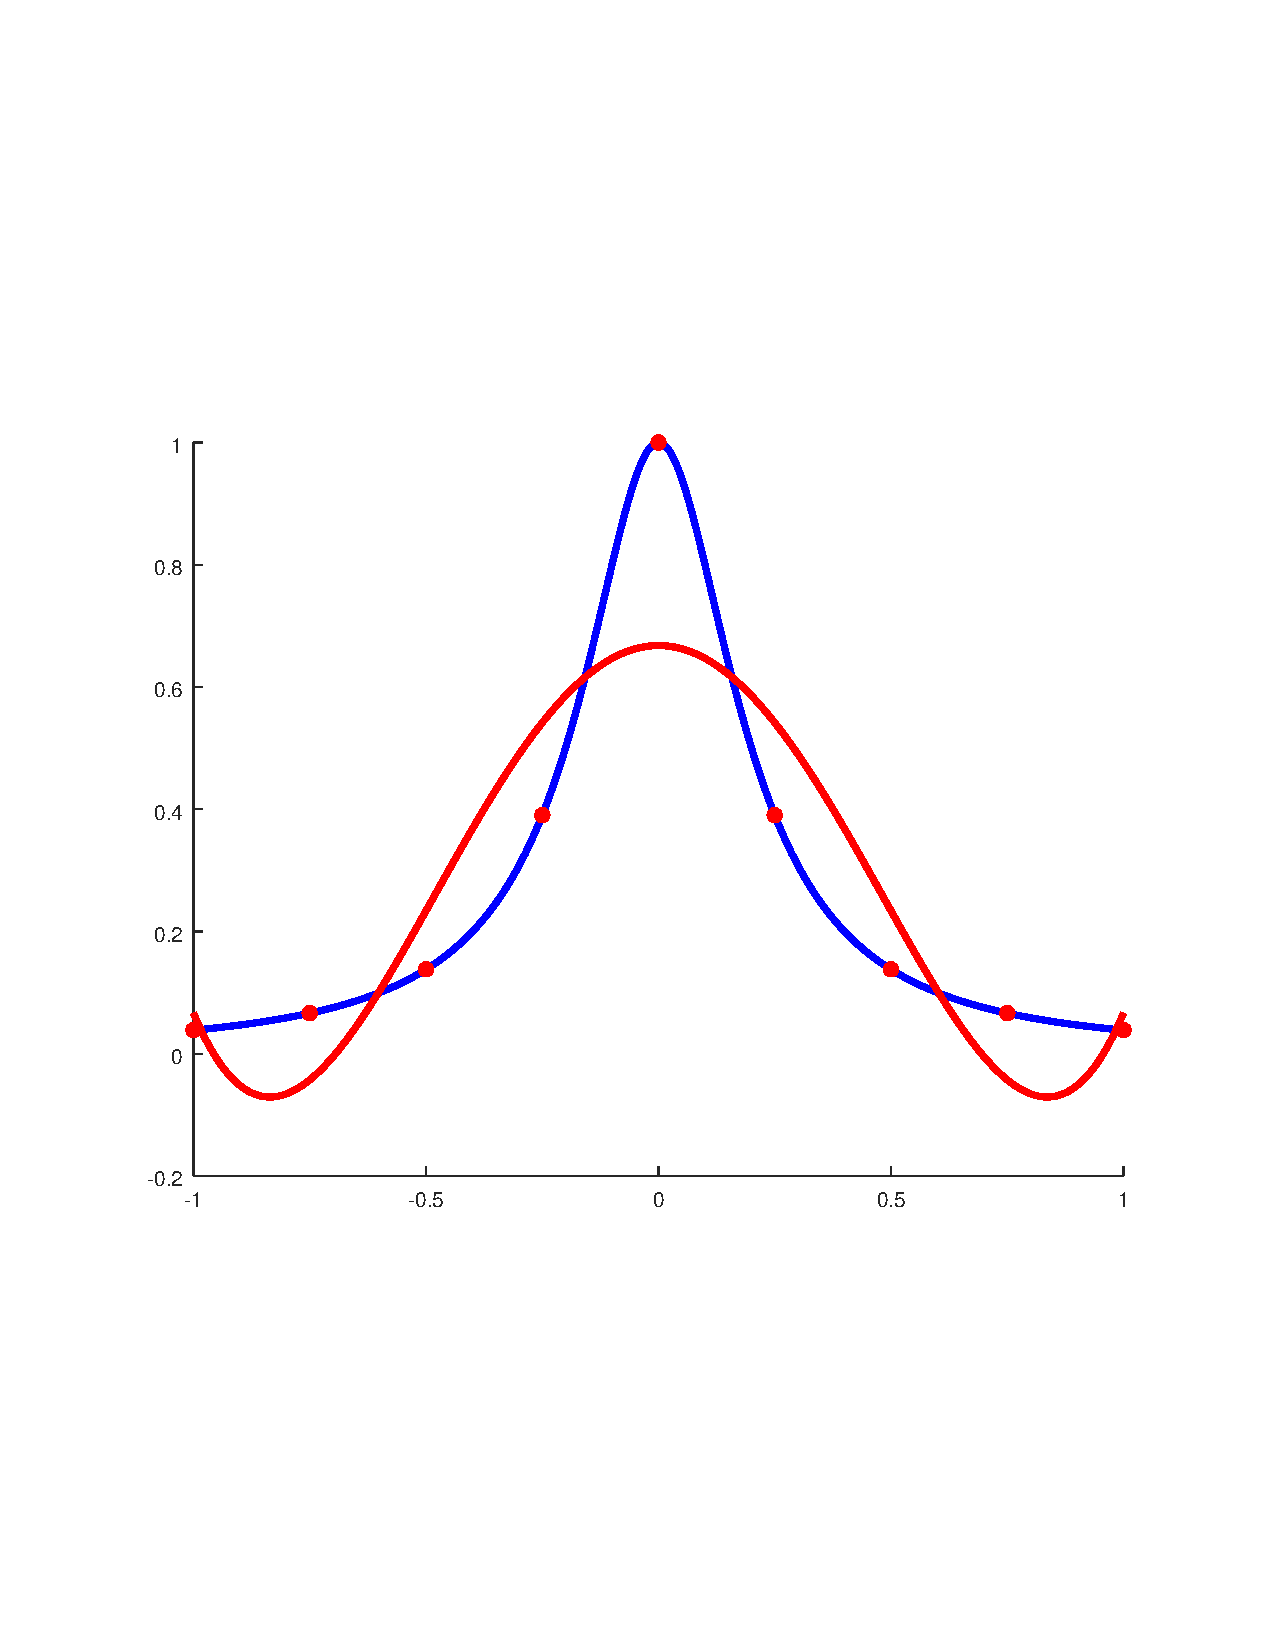
\includegraphics[scale=0.75]{p1}
    {\centering
	    \inputminted[linenos,bgcolor=llgray,frame=lines,framesep=2mm]{octave}{p1.m}}

\problem{}

\begin{enumerate}
    \item Given a point $x_0$ and a step size h, use Lagrange polynomials to find the quadratic polynomial
	    which interpolates a function f(x) at the points $x_0$-2h, $x_0$, and $x_0$+h.
    \item Integrate the polynomial on [$x_0$-2h, $x_0$+h] to produce an integration formula.
	    Use the formula to estimate $\int_{0}^{3} e^{-x} dx$.
\end{enumerate}

\solution

    \part
    \raggedright
    The quadratic Lagrange polynomial P(t) is given by \\
    \begin{align*}
	P(t) &= 
	    f(x_0 - 2h)\frac{(t-t_1)(t-t_2)}{(t_0-t_1)(t_0-t_2)} 
	    + f(x_0)\frac{(t-t_0)(t-t_2)}{(t_1-t_0)(t_1-t_2)} \\
	    &+ f(x_0 + h)\frac{(t-t_0)(t-t_1)}{(t_2-t_0)(t_2-t_1)}
    \end{align*}
    \bigbreak
    In this case we have $t_0 = x_0 - 2h$, $t_1 = x_0$, and $t_2 = x_0 + h$. \\
    Next we make the necessary substitutions and simplify the different parts of P(t). \\
    \begin{align*}
	(t - t_1)(t - t_) &= (t - x_0)(t - (x_0 + h)) &\\
	(t - t_0)(t - t_2) &= (t - x_0 + 2h)(t - x_0 - h) &\\
	(t - t_0)(t - t_1) &= (t - x_0 + 2h)(t - x0) &\\
	(t_0-t_1)(t_0-t_2) &= ((x_0-2h) - x_0)((x_0-2h) - (x_0 + h)) &\\
	&= (-2h)(x_0 - 2h - x_0 - h) &\\
	&= (-2h)(-3h) &\\
	&= 6h^2 &\\
	&= (t - x_0)(t - x_0 - h) &\\
	(t_1-t_0)(t_1-t_2) &= (x_0 - (x_0 - 2h))(x_0 - (x_0 + h)) &\\
	&= (2h)(-h) &\\
	&= -2h^2 &\\
	(t_2 - t_0)(t_2-t_1) &= ((x_0 + h)-(x_0 - 2h))((x_0 - 2h) - x0) &\\
	&= (3h)(h) &\\
	&= 3h^2 &\\
    \end{align*}

    Thus we arrive at the following equation
    \begin{align*}
	P(t) &= 
	    \frac{f(x_0 - 2h)}{6h^2}(t - x_0)(t - x_0 - h)
	    + \frac{f(x_0)}{-2h^2}(t - x_0 + 2h)(t - x_0 - h) \\
	    &+ \frac{f(x_0 + h)}{3h^2}(t - x_0 + 2h)(t - x_0) &\\
	&=
	    \frac{f(x_0 - 2h)}{6h^2}(t^2 - (2x_0 + h)t + (hx_0+x_0^2)
	    + \frac{f(x_0)}{-2h^2}(t^2 + (h-2x_0)t + (x_0^2 - hx_0 - 2h^2) \\
	    &+ \frac{f(x_0 + h)}{3h^2}(t^2 + (2h - x_0)t + (x_0^2 - 2hx_0) &\\
    \end{align*}

    Here we can see the that P(t) is quadratic with respect to t (as expected),
    solving for the coefficients of P(t) = At^2 + Bt + C produces

    \begin{align*}
	A &= f(x_0-2h)\frac{1}{6h^2} + f(x_0)\frac{1}{-2h^2} + f(x_0+h)\frac{1}{3h^2} &\\
	B &= f(x_0-2h)\frac{-2x_0-h}{6h^2} + f(x_0)\frac{h-2x_0}{-2h^2} + f(x_0+h)\frac{2h-2x_0}{3h^2} &\\
	C &= f(x_0-2h)\frac{hx_0 + x_0^2}{6h^2} + f(x_0)\frac{x_0^2 - hx_0 - 2h^2}{-2h^2} 
	    + f(x_0+h)\frac{x_0^2 - 2hx_0}{3h^2} &\\
    \end{align*}

    Note that given h, $x_0$, and the interpolating points $f(x_0-2h)$, $f(x_0)$, and $f(x_0+h)$ each of the
    terms A, B, C are constant with respect to t. \\ 
    Included below is a graph comparing $f(x) = e^{-x}$ with P(t) 
    given $x_0$ = 2, h = 1.

    \bigbreak

    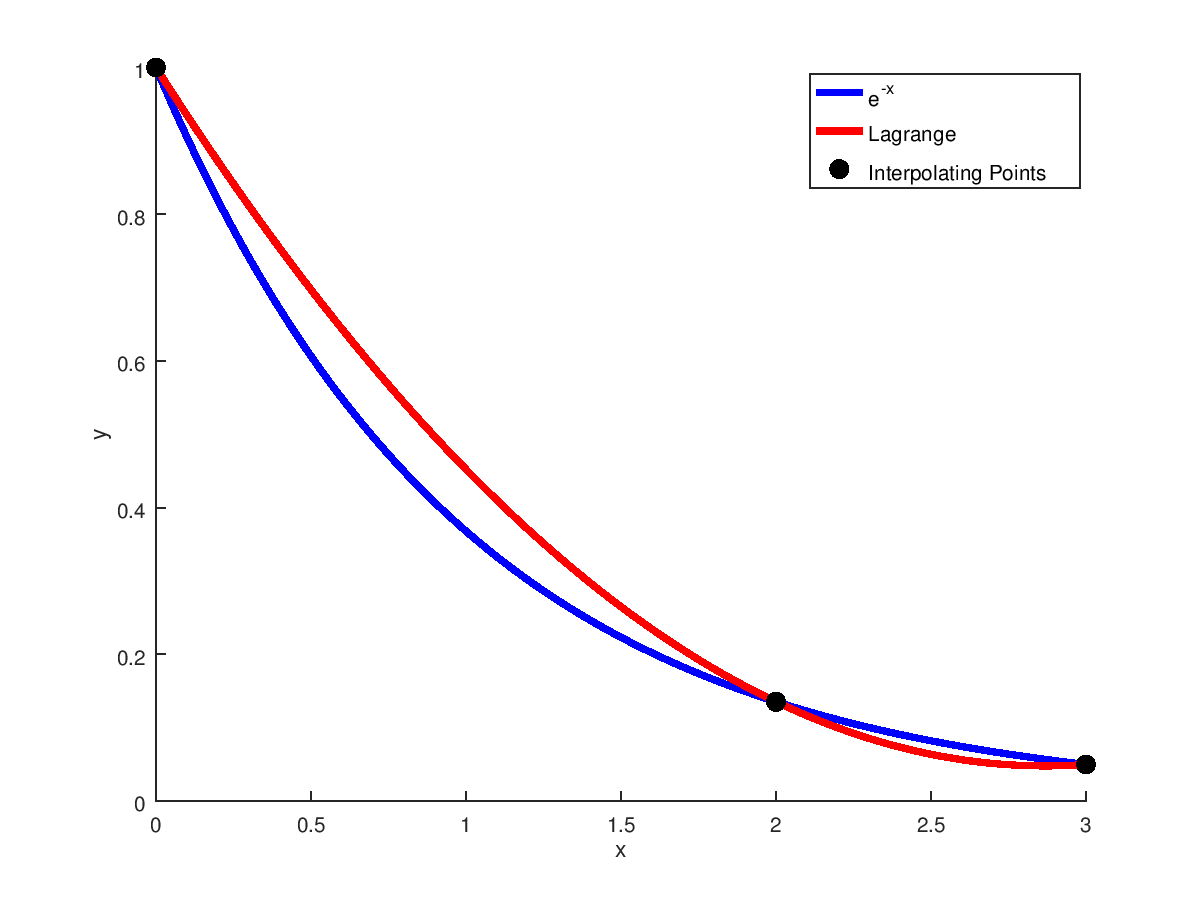
\includegraphics[scale=0.75]{p2}
    \part

    \begin{align*}
	\int_{x_0-2h}^{x_0+h}{P(t)} &= 
	    \int_{x_0-2h}^{x_0+h}{At^2+Bt+C} dt &\\
	&= (\frac{1}{3}At^3 + \frac{1}{2}Bt^2 + Ct) \biggr\rvert_{x_0-2h}^{x_0+h} &\\
	&= (\frac{1}{3}A((x_0+h)^3 - (x_0-2h)^3) + \frac{1}{2}B((x_0+h)^2 -(x_0-2h)^2) + C((x_0+h) - (x_0-2h)) &\\
    \end{align*}

    Expanding and simplifying our terms
    \begin{align*}
	(x_0+h)-(x_0-2h) &= x_0-x_0+h+2h  &\\
	&= 3h &\\
	(x_0+h)^2-(x_0-2h)^2 &= x_0^2 + 2x_0h + h^2 - x_0^2 + 4x_0h - 4h^2 &\\
	&= 6x_0h - 3h^2 &\\
	(x_0+h)^3-(x_0-2h)^3 &= x_0^3 + 3x_0^2h + 3x_0h^2 + h^3 &\\
	&- x_0^3 + 6x_0^2h - 12x_0h^2 + 8h^3 &\\
	&= 9x_0^2 - 9x_0h^2 + 9h^3 &\\
	&= 9(x_0^2h - x_0h^2 + h^3) &\\
    \end{align*}

    This gives us the following equation

    \begin{align*}
	\int_{x_0-2h}^{x_0+h}{P(t)} 
	= 3hA(x_0^2-x_0h+h^2) + \frac{1}{2}hB(6x_0-3h) + C3h
    \end{align*}

    Using the same constant coefficients A, B, C that were derived in part (A). \\
    We can use this formula to estimate $\int_{0}^{3}e^{-x}dx$
    by setting $x_0 = 2$, $h=1$ and plugging those values into our equation for
    $\int_{x_0-2h}^{x_0+h}{P(t)}$. \\
    By doing so we produce the following approximation:

    \begin{align*}
	\int_{0}^{3}P(t)dt &= 1.0545 &\\
	&\approx &\\
	\int_{0}^{3}e^{-x}dx &= 0.95021 &\\
    \end{align*}

    \raggedright
    The estimate of the integral via the Lagrange polynomial has an error of 0.10429.

    {\centering \inputminted[linenos,breaklines,bgcolor=llgray,frame=lines,framesep=2mm]{octave}{p2.m}}

\problem{}

    For k=2, Iserles calls these the Nystrom and Milne methods. That is, start with
    \begin{gather}
	    y(t_{n+2}) = y(t_n) + \int_{t_n}^{t_{n+2}}f(\tau , y(\tau )) d\tau ,
    \end{gather}
    and interpolating at $t_n$, $t_{n+1}$ (explicit) or $t_n$, $t_{n+1}$, $t_{n+2}$ (implicit). \\
    Find the leading error term, and the order of the method, for both cases.

\solution

\part

    Given $y(t_{n+2}) = y(t_n) + \int_{t_n}^{t_{n+2}} f(\tau , y(\tau)) d\tau$, to solve for the explicit
    case (and thus find the error), we must approximate $\int_{t_n}^{t_{n+2}} f(\tau , y(\tau)) d\tau$ using a Lagrange
    polynomial interpolating the points $f(t_n, y_n)$ and $f(t_{n+1}, y(t_{n+1}))$. \\
    That is $y(t_{n+2}) = y(t_n) + \int_{t_n}^{t_{n+2}} f(\tau , 
	y(\tau)) d\tau \approx y(t_n) + \int_{t_n}^{t_{n+2}} P(\tau) d\tau$.
    Where P(t) is the Lagrange polynomial. \\

    \begin{align*}
	P(t) &= f(t_n,y_n)\frac{t-t_{n+1}}{t_n-t_{n+1}} + f(t_{n+1},y(t_{n+1}))\frac{t-t_n}{t_{n+1}-t_n} &\\
	&= \frac{f(t_n,y_n)}{-h}(t-t_{n+1}) + \frac{f(t_{n+1},y(t_{n+1}))}{h}(t-t_n) &\\
    \end{align*}

    Next we integrate each side from $t_n$ to $t_{n+2}$ with respect to t \\

    \begin{align*}
	\int_{t_n}^{t_{n+2}} P(\tau)d\tau
	&=	\frac{f(t_n,y_n)}{-h}\int_{t_n}^{t_{n+2}}(\tau-t_{n+1})d\tau + 
		\frac{f(t_{n+1},y(t_{n+1}))}{h}\int_{t_n}^{t_{n+2}}(\tau-t_n)d\tau &\\
	&=	\frac{f(t_n,y_n)}{-h} (\frac{1}{2}\tau^2 - (t_{n+1})\tau)\biggr\rvert_{t_n}^{t_{n+2}} +
		\frac{f(t_{n+1},y(t_{n+1}))}{h} (\frac{1}{2}\tau^2 - (t_n)\tau)\biggr\rvert_{t_n}^{t_{n+2}}&\\
    \end{align*}

    Evaluating the integrals$\ldots$

    \begin{align*}
	(\frac{1}{2}\tau^2 - (t_{n+1})\tau)\biggr\rvert_{t_n}^{t_{n+2}} &=
		\frac{1}{2}(t_{n+2}^2) - (t_{n+1})(t_{n+2}) - \frac{1}{2}t_n^2 + (t_{n+1})t_n &\\
	    &= \frac{1}{2}(t_{n+2}^2 - t_n^2) + (t_{n+1})(t_n - t_{n+2}) &\\
	    &= \frac{1}{2}(t_{n+2} + t_n)(t_{n+2} - t_n) + -2h(t_{n+1}) &\\
	    &= h(t_{n+2} + t_n) + -2h(t_{n+1}) &\\
	    &= h(t_{n+2} + t_n - t_{n+1} - t_{n+1}) &\\
	    &= h(t_{n+2} - t_{n+1} + t_n - t_{n+1}) &\\
	    &= h(h - h) &\\
	    &= 0 &\\
	(\frac{1}{2}\tau^2-(t_n)\tau)\biggr\rvert_{t_n}^{t_{n+2}} &=
		\frac{1}{2}(t_{n+2})^2 - (t_n)(t_{n+2}) - \frac{1}{2}t_n^2 - (t_{n+1})(t_{n+2}) &\\
	    &= \frac{1}{2}(t_{n+2}^2 - t_n^2) + (t_n)(t_n - t_{n+2}) &\\
	    &= \frac{1}{2}(t_{n+2} + t_n)(t_{n+2} - t_n) + -2h(t_n) &\\
	    &= h(t_{n+2} + t_n) + -2h(t_n) &\\
	    &= h(t_{n+2} + t_n + -t_n - t_n) &\\
	    &= h(t_{n+2}  - t_n) &\\
	    &= h(2h) &\\
    \end{align*}

    Substituting these results into our original equation

    \begin{align*}
	\int_{t_n}^{t_{n+2}} P(\tau)d\tau
	&=	\frac{f(t_n,y_n)}{-h} 0 +
		\frac{f(t_{n+1},y(t_{n+1}))}{h} h(2h) &\\
	&=	2h f(t_{n+1}, y(t_{n+1})) &\\
    \end{align*}

    From 
    \begin{align*}
	y(t_{n+2}) = y(t_n) + \int_{t_n}^{t_{n+2}} f(\tau, y(\tau)) d\tau$ 
	\approx 
	y(t_n) + \int_{t_n}^{t_{n+2}} P(\tau) d\tau = y(t_n) + 2h f(t_{n+1}, y(t_{n+1}))
    \end{align*}
    We get our k-step method as follows
    $$
	y_{n+2} = y_n + 2h f(t_{n+1}, y(t_{n+1})) 
    $$

    The coefficients for the general k-step then are $a_1 = -1, a_1 = 0, b_2 = 0, b_1 = 2, b_0 = 0$.
    Thus $p(w) = w^2 - 1$ and $\sigma(w) = 2w$.

    \begin{align*}
	p(e^h) - h\sigma(e^h) &= e^{2h} - 1 - h2e^h &\\
	    &= \frac{1}{3}h^3 + \frac{1}{3}h^4 + \frac{11}{60}h^5 + \ldots &\\
	    &= \frac{1}{3}h^3 + \BigO{h^4} &\\
    \end{align*}

    This implies that the Nystrom method has order 2, with a leading error term $\frac{1}{3}h^3$.

\part

    \raggedright

    For the implicit case, the Lagrange polynomial approximating $\int_{t_n}^{t_{n+2}} f(\tau , y(\tau)) d\tau$ 
    will use interpolating points $f(t_n, y_n)$, $f(t_{n+1}, y(t_{n+1}))$, and $f(t_{n+2},y(t_{n+2})$. \\
    That is $y(t_{n+2}) = y(t_n) + \int_{t_n}^{t_{n+2}} f(\tau , 
	y(\tau)) d\tau \approx y(t_n) + \int_{t_n}^{t_{n+2}} P(\tau) d\tau$.
    Where P(t) is the Lagrange polynomial. \\

    \begin{align*}
	P(t) &= f(t_n,y(t_n))\frac{(t-t_{n+1})(t-t_{n+2})}{(t_n-t_{n+1})(t_n-t_{n+2})} +
	    f(t_{n+1},y(t_{n+1}))\frac{(t-t_{n})(t-t_{n+2})}{(t_{n+1}-t_n)(t_{n+1}-t_{n+2})} &\\
	    &+ f(t_{n+2},y(t_{n+2}))\frac{(t-t_n)(t-t_{n+1})}{(t_{n+2}-t_n)(t_{n+2}-t_{n+1})}
	&\\
	&= \frac{f(t_n,y(t_n))}{2h^2} (t-t_{n+1})(t-t_{n+2}) +
	    \frac{f(t_{n+1},y(t_{n+1}))}{-h^2} (t-t_{n})(t-t_{n+2}) &\\
	    &+ \frac{f(t_{n+2},y(t_{n+2}))}{2h^2} (t-t_n)(t-t_{n+1}) &\\
    \end{align*}

    Next we integrate P(t)

    \begin{align*}
	\int_{t^n}^{t_{n+2}}P(\tau)d\tau
	    &= \frac{f(t_n,y(t_n))}{2h^2} \int_{t^n}^{t_{n+2}}(\tau-t_{n+1})(\tau-t_{n+2}) d\tau +
	    \frac{f(t_{n+1},y(t_{n+1}))}{-h^2} \int_{t^n}^{t_{n+2}}(\tau-t_{n})(\tau-t_{n+2}) d\tau &\\
	    &+ \frac{f(t_{n+2},y(t_{n+2}))}{2h^2} \int_{t^n}^{t_{n+2}}(\tau-t_n)(\tau-t_{n+1}) d\tau &\\
    \end{align*}

    Where

    \begin{align*}
	\int_{t^n}^{t_{n+2}}(\tau-t_{n+1})(\tau-t_{n+2}) d\tau &= \frac{2}{3}h^3 &\\
	\int_{t^n}^{t_{n+2}}(\tau-t_{n})(\tau-t_{n+2}) d\tau &= -\frac{4}{3}h^3&\\
	\int_{t^n}^{t_{n+2}}(\tau-t_n)(\tau-t_{n+1}) d\tau &= \frac{2}{3}h^3&\\
    \end{align*}

    Thus we have

    \begin{align*}
	\int_{t^n}^{t_{n+2}}P(\tau)d\tau
	    &= \frac{1}{3}hf(t_n,y_n) +
	    \frac{4}{3}hf(t_{n+1},y(t_{n+1})) +
	    \frac{1}{3}hf(t_{n+2},y(t_{n+2})) &\\
    \end{align*}

    Giving us our k-step method
    $$
	y_{n+2} = y_n + 
	    h(\frac{1}{3}f(t_n,y_n) +
	    \frac{4}{3}f(t_{n+1},y_{n+1}) +
	    \frac{1}{3}f(t_{n+2},y_{n+2})) &\\
    $$

    The coefficients for the general k-step then are 
    $a_1 = -1, a_1 = 0, b_2 = \frac{1}{3}, b_1 = \frac{4}{3}, b_0 = \frac{1}{3}$.
    Thus $p(w) = w^2 - 1$ and $\sigma(w) = \frac{1}{3} + \frac{4}{3}w + \frac{1}{3}w^2$.

    \begin{align*}
	p(e^h) - h\sigma(e^h) &= (e^{2h} - 1) - h(\frac{1}{3} + \frac{4}{3}e^h + \frac{1}{3}e^{2h}) &\\
	    &= -\frac{1}{90}h^5 - \frac{1}{90}h^6 - \frac{23}{3780}h^7 \ldots &\\
	    &= -\frac{1}{90}h^5 + \BigO{h^6} &\\
    \end{align*}

    This implies that the Milne method has order 4, with a leading error term -$\frac{1}{90}h^5$.

\problem{}

The IVP \\
\begin{gather}
    y' = -y + e^{-t}$cos(2t)$\\
    y(0) = 0
\end{gather}

has the true solution y(t) = $e^{-t}$sin(2t).
\indent{
    Solve it numerically, using Euler's method with 20, 40, 80, 160 steps from 0 to 1, and compute
    the global error at the endpoint for each stepsize. Verify that the error goes down approximately linearly.
}

\solution

    {\centering
	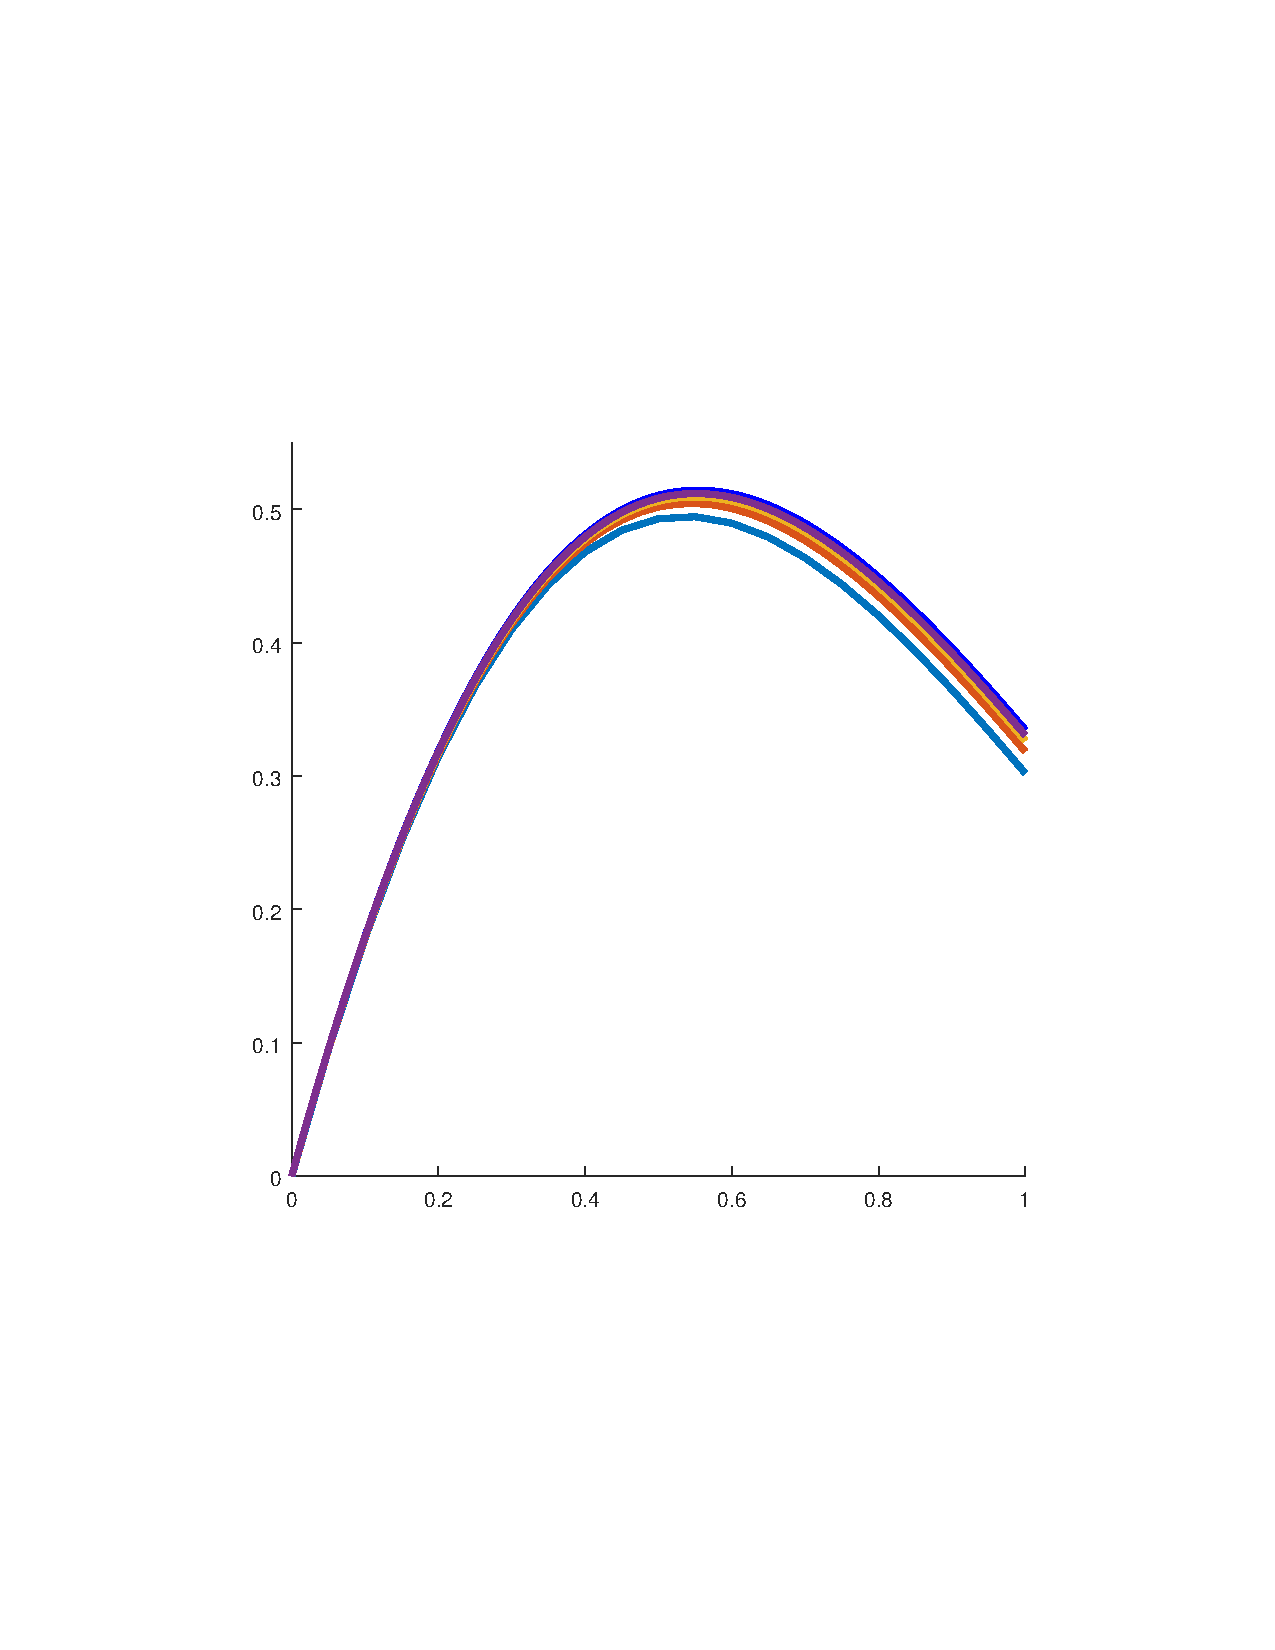
\includegraphics[scale=0.75]{p4} \\
	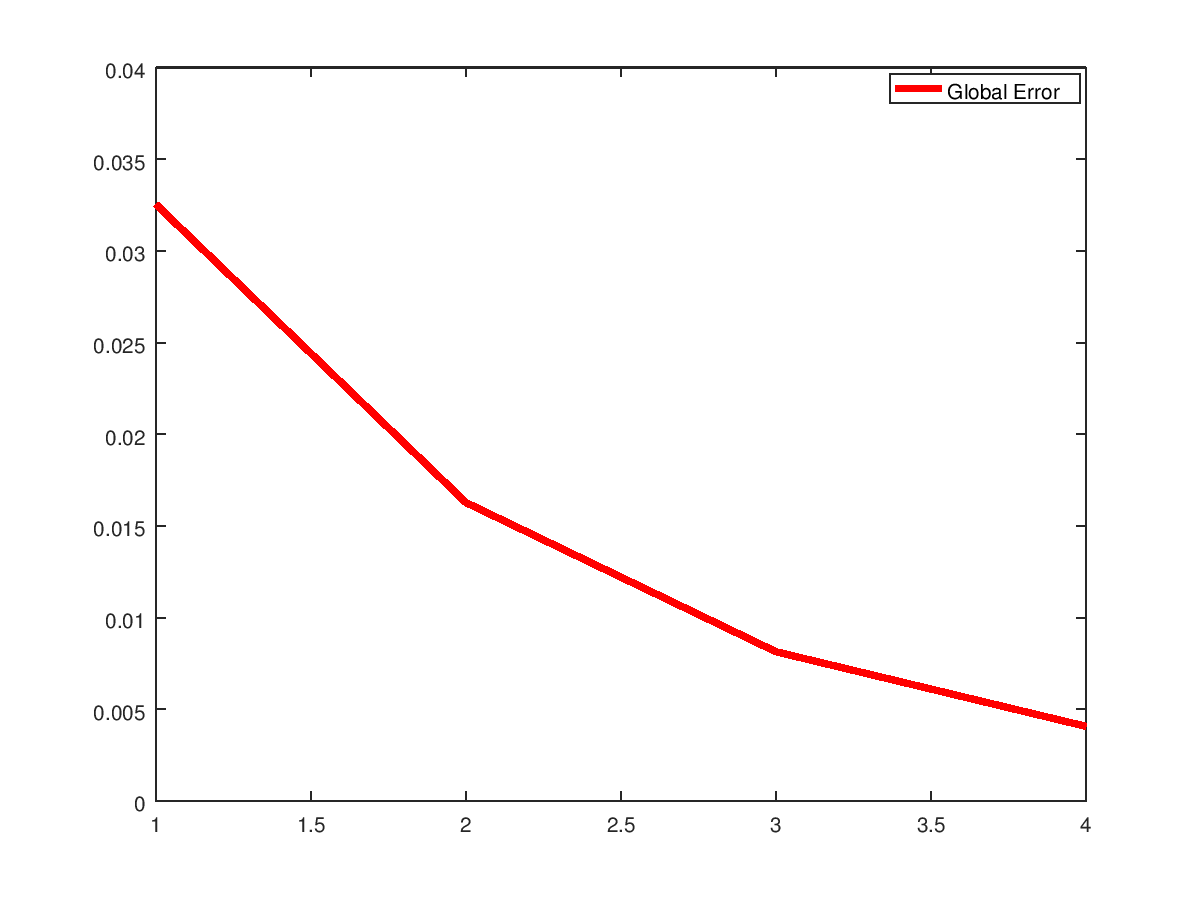
\includegraphics[scale=0.75]{p4_err} \\
    }
    \setlength\parindent{0pt}
    Note that the error term (graphed above) descends approximately linearly with respect to the step size.
    \inputminted[linenos,bgcolor=llgray,frame=lines,framesep=2mm]{octave}{p4.m}

\problem{}

Solve

\raggedright
\setlength\parindent{24pt}
    y''(t) = \begin{bmatrix}0 \\ -10\end{bmatrix} - 0.1y'(t), \\
    \bigbreak
    y(0) = \begin{bmatrix}0 \\ 0\end{bmatrix}$,$ \\
    \bigbreak
    y'(0) = \begin{bmatrix}10 \\ 10\end{bmatrix}
    \bigbreak

\setlength\parindent{0pt}
by using Euler's method with stepsize h = 0.1, until $y_2$ becomes 0 or negative. \\
Plot $y_1$ and $y_)$ as functions of t (horizontal and vertical distance as functions of time), and also
plot $y_2$ versus $y_1$. That will show the path of the object. It should look a bit like a parabola, but compressed
on the right because of friction.

\solution

    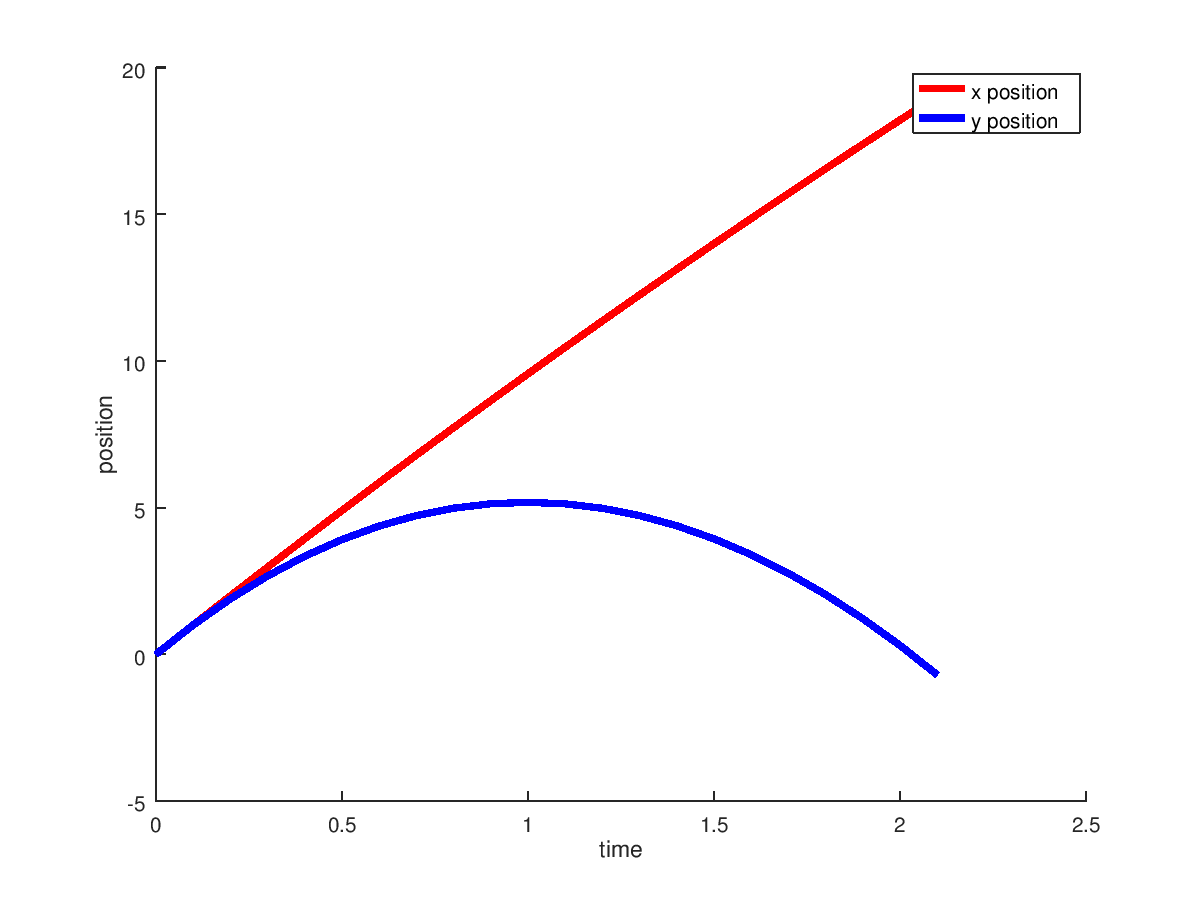
\includegraphics[scale=0.75]{p5_y1_y2_vs_time}
    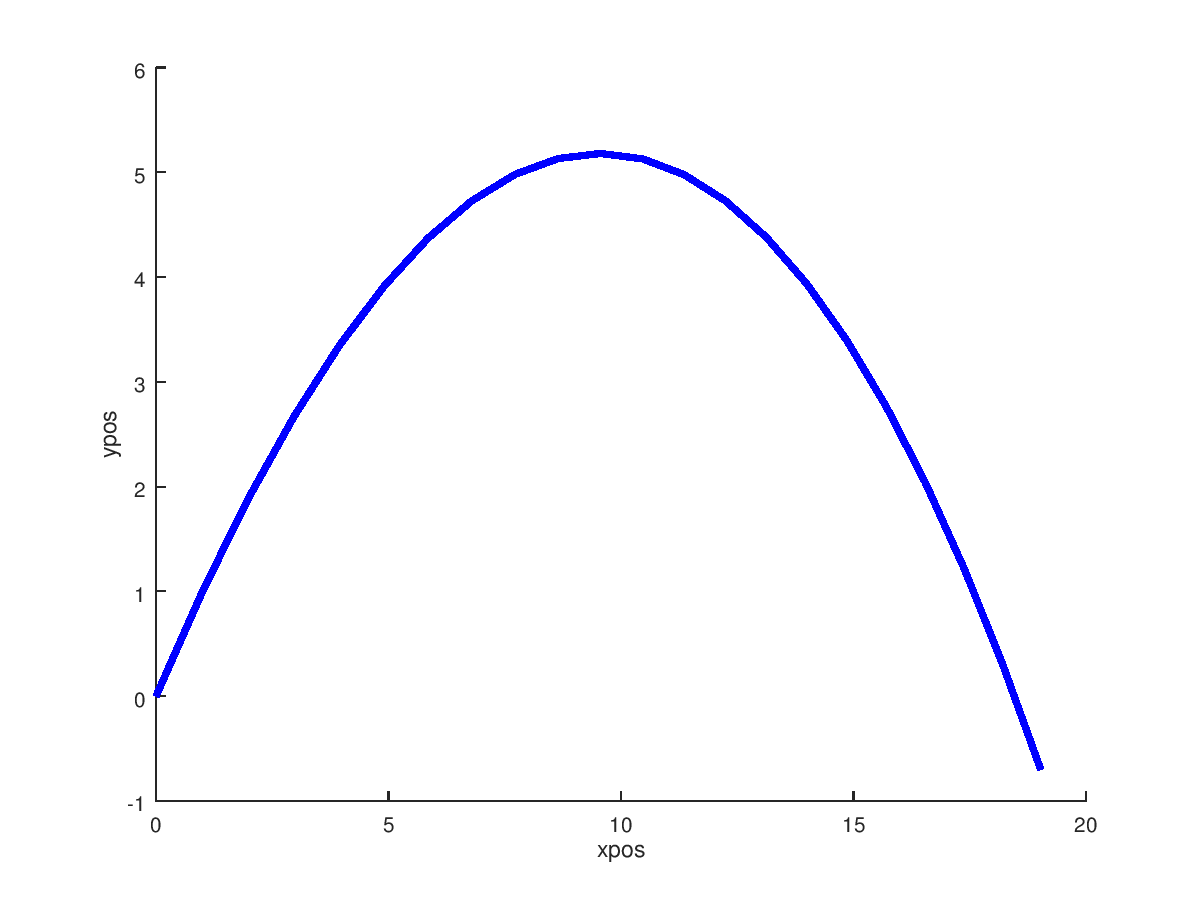
\includegraphics[scale=0.75]{p5}
    {\centering
	    \inputminted[linenos,bgcolor=llgray,frame=lines,framesep=2mm]{octave}{p5.m}}

\end{document}
